In questa sezione vengono delineati i concetti chiave alla base dell'applicazione, la sua vision e i requisiti principali che guidano lo sviluppo del progetto.
Inoltre, viene presentata un'analisi dei competitor per comprendere meglio il contesto di mercato e identificare le opportunità di differenziazione.

\section{System concept statement}
\label{sec:system-concept-statement}

Vivo è un'applicazione mobile progettata per supportare giovani e adulti che desiderano gestire l'ansia e gli attacchi di panico in modo efficace, con l'intento di disinnescare i meccanismi che li alimentano e tornare a vivere a pieno (da qui la scelta del nome \enquote{Vivo}).
La società moderna, con le sue costanti pressioni e sfide quotidiane, genera frequentemente livelli significativi di stress, portando molte persone a sentirsi sopraffatte e vulnerabili di fronte alle proprie difficoltà emotive.
L'applicazione interviene in queste situazioni offrendo strumenti pratici e un supporto immediato, accessibile in qualsiasi momento.
La presenza di un diario personale integrato, inoltre, permette agli utenti di monitorare il proprio percorso di crescita, riflettere sulle esperienze vissute e agevolare la condivisione dei propri stati d'animo con amici, familiari o professionisti.
Favorendo una maggiore consapevolezza di sé, l'app si configura come un vero e proprio compagno digitale per la promozione del benessere mentale e della resilienza.
L'esperienza utente offerta è intuitiva, rassicurante e user-friendly: attraverso un'interfaccia chiara e ottimizzata, l'utente è facilitato nella navigazione, garantendo un'interazione sicura che lo aiuta ad affrontare le fasi critiche con serenità.

\section{Competitive assessment}
\label{sec:competitive-assessment}

In questa sezione viene presentata un'analisi dei competitor, con l'obiettivo di comprendere meglio il contesto di mercato e identificare le opportunità di differenziazione per l'applicazione Vivo.
L'analisi si concentra su due applicazioni principali che affrontano tematiche simili, valutando le loro caratteristiche, punti di forza e debolezze.

\subsection{Rootd}
\label{subsec:rootd}

L'esperienza utente di Rootd si apre con una fase di onboarding orientata alla profilazione tramite domande preliminari, sebbene l'applicazione non sembri restituire un chiaro utilizzo di questi dati in termini di personalizzazione del servizio.
Fin dalle prime schermate, il sistema evidenzia il supporto dell'Università di Victoria, una scelta progettuale efficace per conferire autorevolezza e credibilità.
Il processo è guidato dalla mascotte digitale Ron, un avatar azzurro che tenta di rendere l'interazione più umana ma che fatica a trasmettere un'adeguata sensazione di calma.
Il setup iniziale risulta eccessivamente lungo e genera un'evidente barriera per l'utenza europea, in quanto il sistema propone opzioni di accesso legate a cliniche o assicurazioni sanitarie tipicamente statunitensi.
Questa fase si conclude con un paywall aggressivo che blocca l'accesso immediato, introducendo un ostacolo strutturale (\textit{friction}) che penalizza l'accessibilità per chi si trova in una situazione di crisi.

Dal punto di vista dell'architettura visiva, la home page presenta un layout essenziale.
Nella sezione superiore è posizionato l'avatar di Ron, affiancato da un indicatore dello stato emotivo.
La mascotte funge anche da assistente conversazionale basato su AI, sebbene tale funzionalità sia vincolata alla sottoscrizione di un abbonamento.
L'area centrale presenta una serie di pulsanti che consentono di avviare rapidamente diverse attività di supporto.
All'interno della barra di navigazione, l'applicazione include una sezione dedicata alle statistiche che permette di visualizzare il tempo trascorso nelle attività, l'avanzamento in specifiche lezioni e un calendario settimanale dell'umore.
Questa stessa sezione ospita le impostazioni generali.

L'elemento centrale della barra di navigazione è il pulsante per richiedere aiuto.
Nonostante la sua funzione critica, a questo comando è stata attribuita un'errata gerarchia visiva, poiché è stato inserito tra i normali elementi di navigazione e, pur essendo accompagnato da un'etichetta a forma di fumetto con la scritta \enquote{Start here}, risulta ambiguo e non fa comprendere chiaramente a cosa si riferisca.
A questo errore progettuale si somma la scelta del colore rosso, che risulta disfunzionale al contesto d'uso in quanto rischia di indurre un inutile senso di allarme anziché fornire rassicurazione visiva.
Oltre ai difetti visivi che rischiano di generare sovraccarico cognitivo in un momento critico, il flusso di soccorso risulta funzionalmente limitato.
In caso di attacco di panico, il percorso offre esclusivamente la lettura di frasi di conforto e un audio guidato, omettendo strumenti fondamentali come esercizi di respirazione o tecniche di grounding (pur essendo questi presenti in altre sezioni dell'app).
Un'ulteriore criticità di interazione riguarda il tracciamento dei dati.
L'utente non ha la possibilità di registrare il proprio stato emotivo e i relativi inneschi durante la richiesta di aiuto, ma può farlo esclusivamente nei momenti di calma, perdendo così l'opportunità di contestualizzare lo stato d'animo legato all'attacco.

\begin{figure}[htbp]
    \centering
    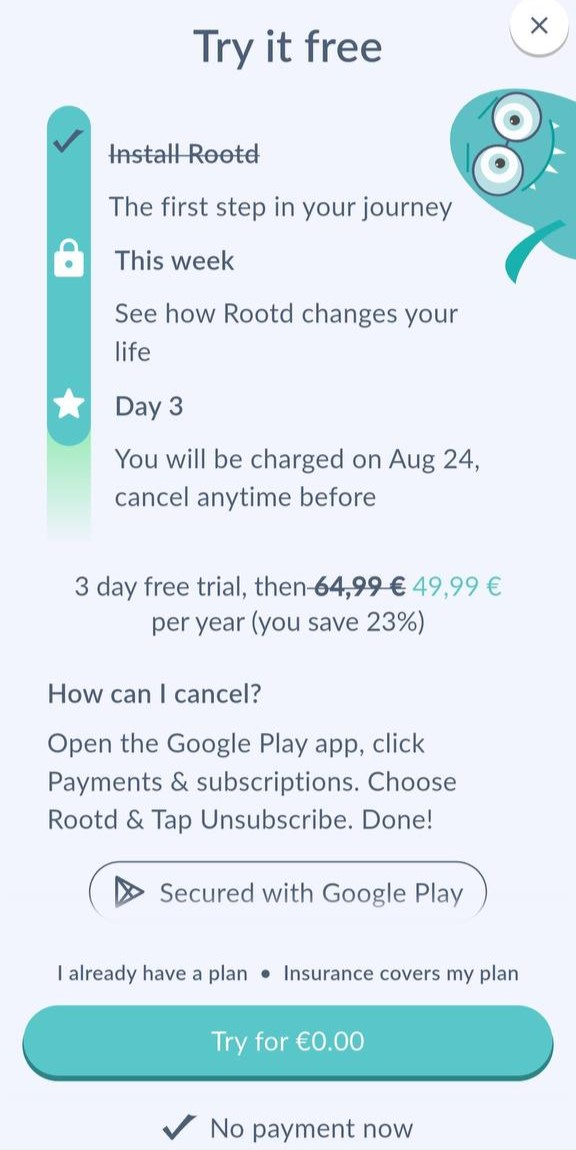
\includegraphics[height=7.5cm]{imgs/envision/rootd/paywall.jpg}\hfill
    
\includegraphics[height=7.5cm]{imgs/envision/rootd/homepage.jpg}\hfill
    
\includegraphics[height=7.5cm]{imgs/envision/rootd/request.jpg}
    \caption{Rootd: il paywall che chiude l'onboarding, la schermata principale e il percorso di richiesta di aiuto}
    \label{fig:rootd}
\end{figure}

\subsection{Dare}
\label{subsec:dare}

L'esperienza utente di Dare si apre con un processo di onboarding decisamente meno invasivo rispetto a Rootd.
L'utente ha infatti la possibilità di saltare la profilazione iniziale e accedere direttamente alla home page.
Tuttavia, superata questa fase, l'interfaccia si presenta fin da subito affetta da criticità legate all'architettura dell'informazione.
La schermata principale ospita una griglia di pulsanti relativi a diverse problematiche come ansia, attacchi di panico e insonnia.
Questi elementi risultano aggregati senza un chiaro criterio di categorizzazione.
All'interno di questo stesso gruppo è inserito un pulsante di SOS di colore rosso che perde di efficacia visiva fondendosi nel layout generale senza il necessario isolamento spaziale.

Dal punto di vista dell'architettura visiva, la barra di navigazione inferiore si articola in cinque macro aree: la home, la sezione relax, il pulsante di emergenza, le sfide giornaliere e la gestione del profilo.
La presenza di un comando di SOS dedicato all'interno di questa barra genera una ridondanza funzionale rispetto all'analogo pulsante inserito nella schermata principale.
Inoltre, analogamente a quanto osservato nel competitor precedente, il flusso di soccorso risulta funzionalmente limitato.
Il percorso di emergenza offre esclusivamente audio guidati e frasi di conforto, omettendo totalmente strumenti pratici e interattivi per la gestione attiva dell'attacco di panico.

L'esplorazione verticale della home page evidenzia un notevole sovraccarico cognitivo.
La pagina è infatti saturata con contenuti eterogenei e disconnessi tra loro, come storie di successo, frasi ispirazionali, webinar e dinamiche social.
Questa frammentazione genera un layout destrutturato che rende l'esperienza d'uso poco intuitiva e ostacola la reperibilità delle informazioni persino in situazioni di totale calma emotiva.
A questo rumore visivo si aggiungono barriere di navigazione legate alla registrazione e alla monetizzazione.
Un banner permanente che invita all'attivazione del free trial è ancorato in modo invasivo appena sopra la barra di navigazione, mentre l'accesso all'assistente conversazionale basato su AI e a molte attività della sezione relax risulta bloccato agli utenti non registrati.

\begin{figure}[htbp]
    \centering
    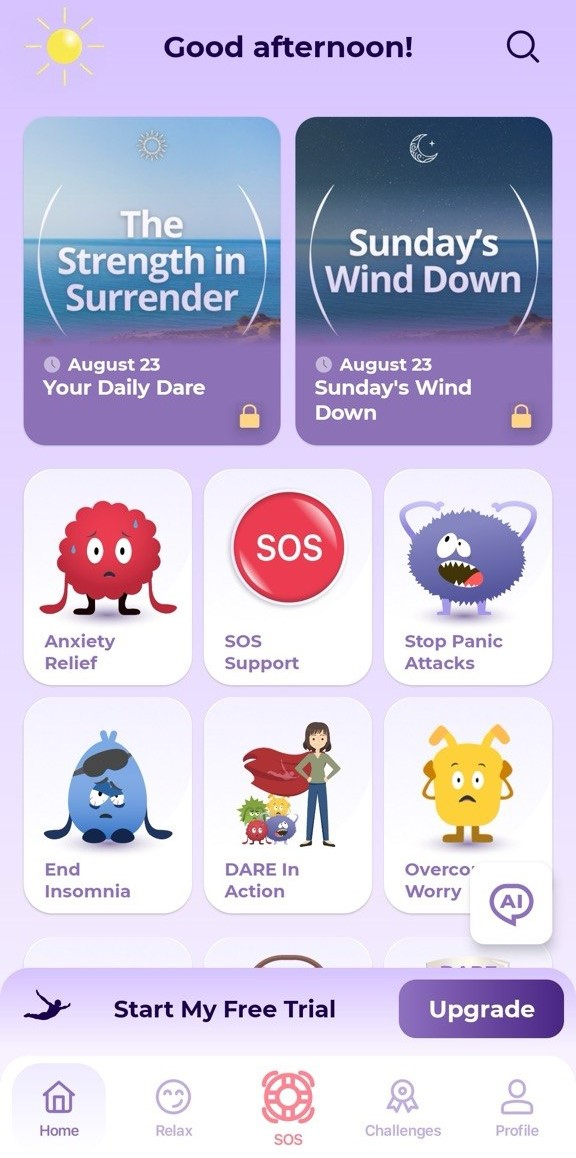
\includegraphics[height=7.5cm]{imgs/envision/dare/homepage.jpg}\hfill
    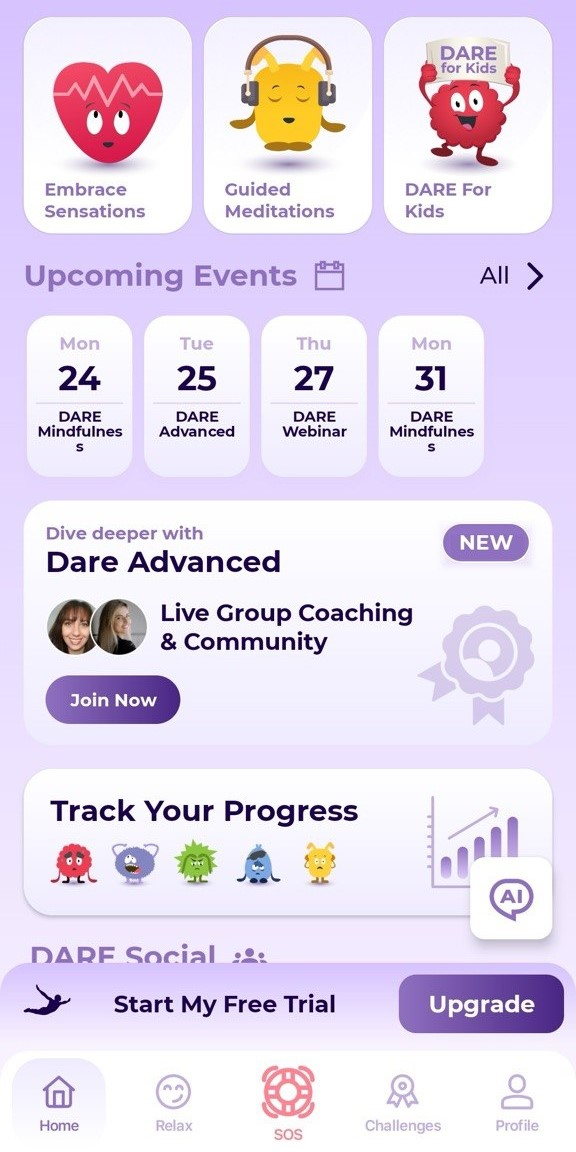
\includegraphics[height=7.5cm]{imgs/envision/dare/scrolled.jpg}\hfill
    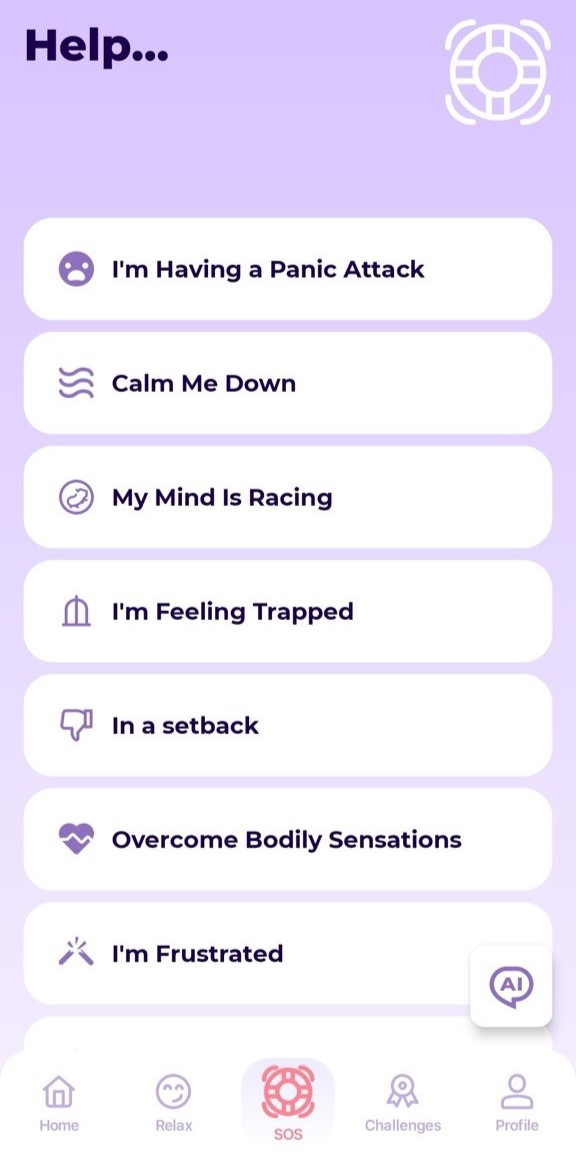
\includegraphics[height=7.5cm]{imgs/envision/dare/request.jpg}
    \caption{Dare: la schermata principale, la stessa pagina scorsa verso il basso e il percorso di emergenza}
    \label{fig:dare}
\end{figure}

\subsection{Sintesi comparativa e posizionamento strategico}
\label{subsec:sintesi-comparativa}

I risultati dell'analisi competitiva sono stati sintetizzati nella tabella seguente, che mette a confronto le due applicazioni esaminate con la proposta di Vivo.
I criteri scelti non sono valutazioni complessive ma fatti osservabili nelle schermate riportate sopra, cosicché il confronto resti verificabile da chi legge e non richieda di fidarsi del giudizio di chi scrive.
Le righe individuano insieme le carenze del mercato e i punti su cui il progetto si differenzia.

\begin{table}[htbp]
    \centering
    \small
    \renewcommand{\arraystretch}{1.3}
    \begin{tabularx}{\textwidth}{L{3.1cm} X X X}
        \toprule
        \textbf{Criterio di confronto} & \textbf{Rootd} & \textbf{Dare} & \textbf{Vivo} \\
        \midrule
        Accesso agli strumenti al primo avvio & Onboarding lungo seguito da paywall & Onboarding saltabile & \textbf{Immediato} \\
        Registrazione richiesta & Sì & Per una parte delle funzioni & \textbf{No} \\
        Esercizi attivi nel percorso di emergenza & Assenti, solo frasi di conforto e audio guidato & Assenti, solo frasi di conforto e audio guidato & \textbf{Respirazione guidata, distrazione cognitiva e grounding} \\
        Collocazione del comando di emergenza & Nella barra di navigazione, fra gli altri elementi & Duplicato fra schermata principale e barra di navigazione & \textbf{Unico, nella schermata principale} \\
        Carico informativo della schermata principale & Contenuto, con elementi di lettura ambigua & Elevato, contenuti eterogenei in sequenza & \textbf{Ridotto al minimo} \\
        Registrazione dello stato emotivo & Solo a freddo, slegata dall'episodio & Solo a freddo, slegata dall'episodio & \textbf{Contestuale, al termine della crisi} \\
        Conservazione dei dati & Account con sincronizzazione remota & Account con sincronizzazione remota & \textbf{Solo sul dispositivo} \\
        Modello di business & Freemium, con paywall bloccante & Freemium, con banner permanente & \textbf{Gratuito, senza pubblicità} \\
        \bottomrule
    \end{tabularx}
    \caption{Confronto fra i competitor analizzati e la proposta di Vivo}
    \label{tab:competitor}
\end{table}

Le righe della tabella si lasciano raggruppare in tre lacune, che sono poi i tre punti su cui il progetto si costruisce.

\textbf{Il soccorso è passivo.}
Entrambe le applicazioni rispondono al momento della crisi con qualcosa da leggere o da ascoltare, ovvero frasi di conforto e audio guidati, e collocano altrove gli esercizi che agirebbero sul corpo e sull'attenzione.
Chi apre l'applicazione durante un attacco di panico riceve così un contenuto da seguire con la mente proprio quando la mente è meno disponibile.
Vivo colloca al centro del percorso di emergenza tre attività da fare, non da leggere.

\textbf{L'aiuto sta dietro una barriera.}
Il primo avvio di Rootd chiede una profilazione lunga e si chiude con un paywall, mentre Dare consente di saltare l'onboarding ma riserva agli utenti registrati una parte delle funzioni.
In entrambi i casi l'ostacolo si presenta nel punto in cui la persona ha bisogno di aiuto immediato, e un ostacolo in quel punto equivale all'assenza dello strumento.
Vivo rende raggiungibile il percorso di soccorso al primo avvio, senza account e senza pagamenti.

\textbf{Il tracciamento è scollegato dall'episodio.}
In nessuna delle due applicazioni è possibile registrare lo stato emotivo e la causa scatenante nel momento in cui la crisi si conclude, e la registrazione resta confinata ai momenti di calma.
Il risultato è un archivio che dice come è andata la giornata ma non che cosa è successo durante l'attacco.
Vivo chiude ogni sessione con un questionario breve e riporta quanto raccolto nella giornata corrispondente del diario.

A queste si aggiunge una differenza di impostazione più che di funzione, poiché i contenuti dei competitor vivono su un account sincronizzato con un servizio remoto, mentre in Vivo restano sul dispositivo e non vengono scambiati con nulla.

\section{Personas}
\label{sec:personas}

L'analisi dei competitor ha messo in luce quali bisogni il mercato lascia scoperti, ma non dice ancora chi sia la persona che li prova.
Sono stati perciò definiti due profili utente, ciascuno dei quali raccoglie in una figura verosimile un modo ricorrente di incontrare l'applicazione.
I due profili non sono intercambiabili.
Il primo incontra Vivo nel momento della crisi e ne mette alla prova l'immediatezza, il secondo lo utilizza nei giorni in cui sta bene e ne mette alla prova la capacità di restituire un andamento leggibile nel tempo.
Mantenere presenti entrambe le figure durante la progettazione evita che l'applicazione si sbilanci verso una sola di esse, riducendosi a un pulsante di emergenza privo di memoria oppure a un diario che nel momento dell'attacco non offre alcun aiuto.

\begin{table}[htbp]
    \centering
    \small
    \renewcommand{\arraystretch}{1.3}
    \begin{tabularx}{\textwidth}{L{3.4cm} X}
        \toprule
        \multicolumn{2}{c}{\textbf{Persona 1: Giulia Rossi}} \\
        \midrule
        Età & 21 anni \\
        Occupazione & Studentessa universitaria fuorisede, iscritta al secondo anno \\
        Contesto & I primi attacchi di panico sono comparsi durante la sessione invernale e oggi si ripresentano in situazioni difficili da prevedere, in aula affollata o sui mezzi pubblici \\
        Percorso di cura & Nessuno, non ne ha parlato con uno specialista perché non ritiene il proprio caso abbastanza serio \\
        Rapporto con la tecnologia & Elevato, tiene lo smartphone sempre a portata di mano e ha già scaricato e disinstallato due applicazioni del settore \\
        Obiettivi & Uscire dalla crisi mentre questa è ancora in corso, ricevendo un'indicazione operativa su cosa fare e non una frase di conforto da leggere. Raggiungere lo strumento in pochi secondi e poterlo usare in luoghi pubblici senza dare nell'occhio. Riconoscere, a crisi conclusa, che cosa l'abbia scatenata, senza compilare moduli lunghi \\
        Frustrazioni & Procedure di onboarding estese e domande di profilazione poste prima di poter usare l'applicazione. Registrazione obbligatoria per accedere agli strumenti di emergenza. Paywall collocato proprio sulla funzione di cui avrebbe avuto bisogno \\
        \bottomrule
    \end{tabularx}
    \caption{Prima persona: chi incontra l'applicazione nel momento della crisi}
    \label{tab:persona1}
\end{table}

\begin{table}[htbp]
    \centering
    \small
    \renewcommand{\arraystretch}{1.3}
    \begin{tabularx}{\textwidth}{L{3.4cm} X}
        \toprule
        \multicolumn{2}{c}{\textbf{Persona 2: Marco Bianchi}} \\
        \midrule
        Età & 38 anni \\
        Occupazione & Impiegato amministrativo, lavora a tempo pieno \\
        Contesto & Convive con un disturbo d'ansia da diversi anni e attraversa periodi in cui gli attacchi si concentrano in poche settimane, seguiti da mesi più tranquilli \\
        Percorso di cura & Segue un percorso psicoterapeutico con incontri ogni due settimane \\
        Rapporto con la tecnologia & Medio, usa poche applicazioni ma con costanza, e diffida di quelle che richiedono di affidare i propri dati a un servizio esterno \\
        Obiettivi & Annotare che cosa accade durante e dopo un attacco, per poterlo riferire con precisione nella seduta successiva. Osservare l'andamento del proprio stato nel tempo e capire se il periodo in corso sia migliore o peggiore del precedente. Praticare gli esercizi di respirazione e di grounding anche nei momenti di calma, per averne padronanza quando serviranno davvero. Mettere per iscritto quello che prova, senza doverlo far rientrare in una scala di valori prestabilita \\
        Frustrazioni & Ricostruire a memoria, giorni dopo, un episodio di cui sul momento aveva chiare tutte le circostanze. Dati intimi conservati su server esterni, dei quali non conosce la destinazione. Riepiloghi che si limitano a elencare le registrazioni passate senza indicare alcuna tendenza. Dimenticare di annotare la giornata proprio nei periodi in cui il tracciamento sarebbe più utile \\
        \bottomrule
    \end{tabularx}
    \caption{Seconda persona: chi utilizza l'applicazione come strumento di osservazione nel tempo}
    \label{tab:persona2}
\end{table}

\section{Requirements brief e prioritizzazione}
\label{sec:requirements-brief}

Sulla base della vision, delle opportunità individuate nell'analisi dei competitor e dei bisogni delle due personas appena descritte sono stati definiti i requisiti del sistema.
Ciascuno di essi è formulato come qualcosa che l'utente può fare con l'applicazione, e non come un componente da costruire, poiché un elenco di componenti non dice nulla su ciò che la persona ottiene e rende impossibile stabilire se il requisito sia stato soddisfatto.
A ogni requisito è associato un livello di priorità, stabilito in base al suo impatto sulla User Experience e alla sua rilevanza rispetto all'obiettivo principale di offrire un supporto immediato ed efficace nella gestione dell'ansia e degli attacchi di panico.

\subsection{Must-have requirements}
\label{subsec:must-have}

\begin{itemize}
    \item \textbf{REQ-01: Capire a colpo d'occhio che cosa fare in ogni schermata.} L'utente può individuare l'azione principale di una schermata senza leggere istruzioni e senza dover scegliere fra elementi visivamente equivalenti, poiché ogni schermata espone un solo comando dominante e nessun contenuto estraneo al proprio scopo. A questo requisito è assegnata una priorità alta poiché in momenti di forte vulnerabilità emotiva o durante un attacco di panico un'interfaccia complessa o caotica genera un immediato sovraccarico cognitivo che ostacola l'accesso agli strumenti di soccorso.

    \item \textbf{REQ-02: Fare qualcosa durante la crisi, non soltanto leggere.} L'utente può svolgere, mentre l'attacco è in corso, esercizi guidati che agiscono sul respiro con la tecnica 4-4-4-4, sull'attenzione con un'attività di distrazione cognitiva e sui sensi con la tecnica di grounding. La priorità è alta in quanto questi strumenti rappresentano il fulcro funzionale di Vivo. Questo requisito colma la principale lacuna dei competitor, superando l'inefficacia della sola lettura di frasi di conforto.

    \item \textbf{REQ-03: Uscire da qualsiasi percorso sapendo che cosa comporta.} L'utente può interrompere in ogni momento un'attività o una schermata e tornare alla schermata principale, e prima che l'abbandono avvenga il sistema gli dichiara le conseguenze della scelta, in particolare quando interrompere un percorso significa non conservarne il contenuto. Fanno eccezione le brevi schermate di passaggio, che non trattengono l'utente perché si esauriscono da sole dopo pochi secondi e possono essere accelerate con un tocco. La priorità è alta poiché durante una crisi d'ansia la percezione di sentirsi bloccati in un flusso irreversibile genera disorientamento e profonda frustrazione, rischiando di alimentare ulteriormente lo stato di panico.

    \item \textbf{REQ-04: Raggiungere gli strumenti di emergenza fin dal primo avvio.} L'utente può arrivare al percorso di aiuto senza creare un account, senza completare una procedura di configurazione iniziale e senza superare alcun pagamento. Questo requisito ha una priorità alta poiché, come emerso dall'analisi dei competitor, i registration wall e i setup prolungati rappresentano ostacoli critici (\textit{friction}) che impediscono un intervento tempestivo nel momento del bisogno.

    \item \textbf{REQ-05: Sapere che i propri contenuti restano sul telefono e poterli cancellare.} L'utente può registrare dati anagrafici, riflessioni e storico delle crisi con la garanzia che nulla venga trasmesso verso server esterni, e chi ha creato un profilo può eliminare l'intero archivio in qualsiasi momento. A chi sceglie di usare l'applicazione come ospite, e quindi non ha un profilo da eliminare, resta la disinstallazione, che cancella ugualmente ogni contenuto. La priorità è alta poiché il materiale raccolto è tra i più intimi che una persona possa affidare a un'applicazione, e il solo sospetto che quei contenuti possano essere letti altrove indurrebbe l'utente a censurarsi proprio nei momenti in cui la scrittura sincera ha maggiore valore terapeutico.
\end{itemize}

\subsection{Should-have requirements}
\label{subsec:should-have}

\begin{itemize}
    \item \textbf{REQ-06: Registrare come sta e che cosa ha scatenato l'attacco.} L'utente può segnare il proprio stato d'animo giornaliero e, al termine di una sessione di aiuto, dichiarare l'intensità dell'attacco appena affrontato e il fattore che lo ha innescato. La priorità è media, poiché si tratta di una funzione che non interviene nell'emergenza immediata, ma risulta fondamentale nel medio periodo per aiutare l'utente a sviluppare consapevolezza emotiva e prevenire crisi future.

    \item \textbf{REQ-07: Rileggere le proprie giornate passate.} L'utente può consultare lo storico e ritrovare, per ciascun giorno, l'umore registrato, le richieste di aiuto con l'orario, l'intensità e il fattore scatenante di ciascuna, e la riflessione scritta. La priorità è media poiché questa funzione consente all'utente di riflettere sul proprio percorso di crescita, monitorare l'evoluzione dell'ansia tra una crisi e l'altra e avere un quadro chiaro da consultare in autonomia.

    \item \textbf{REQ-08: Praticare un esercizio anche quando sta bene.} L'utente può avviare singolarmente la respirazione guidata e il grounding, in un momento qualsiasi e senza attivare l'intero percorso di soccorso. La priorità è media poiché questa possibilità sposta gli strumenti dal solo momento della crisi alla quotidianità, permettendo di gestire gli stati di ansia lieve o anticipatoria e di prendere confidenza con le tecniche in un momento di calma: un esercizio già praticato si esegue con maggiore facilità quando le capacità cognitive sono ridotte dal panico.

    \item \textbf{REQ-09: Vedere se la settimana è andata meglio della precedente.} L'utente può leggere, senza doverlo calcolare, quante volte ha chiesto aiuto nella settimana corrente, quante nella settimana precedente e di quanto il dato sia cambiato. La priorità è media poiché questa sintesi non incide sulla gestione dell'emergenza, ma trasforma una sequenza di registrazioni isolate in un andamento leggibile a colpo d'occhio, restituendo all'utente la percezione concreta del proprio miglioramento e sostenendo la motivazione a proseguire il percorso.

    \item \textbf{REQ-10: Scrivere liberamente ciò che prova.} L'utente può annotare un testo senza vincoli di formato, di lunghezza o di argomento, legato al singolo giorno, e può riaprirlo e modificarlo anche in un momento successivo. La priorità è media poiché la scrittura non interviene durante l'attacco, quando articolare un pensiero è già di per sé faticoso, ma nelle ore che lo seguono consente di dare un nome a ciò che si è provato: mettere in parole un'esperienza confusa la rende più maneggiabile e, a differenza di un valore scelto da una scala predefinita, non costringe il vissuto dell'utente entro categorie stabilite da altri.

    \item \textbf{REQ-11: Avere un profilo personale e tenerne aggiornati i dati.} L'utente può creare un profilo con nome, cognome, indirizzo di posta elettronica, data di nascita, genere e immagine, correggere in seguito ciascuna di queste informazioni, cambiare la propria password e disconnettersi dal dispositivo. La priorità è media poiché l'applicazione resta pienamente utilizzabile anche senza profilo, come stabilito dal requisito di accesso senza barriere (\textbf{REQ-04}), ma chi sceglie di crearne uno le affida dei dati che devono restare correggibili senza ricominciare da capo, mentre la disconnessione e il cambio della password sono ciò che permette di tenere il diario al riparo su un telefono che capita di lasciare in mano ad altri.
\end{itemize}

\subsection{Could-have requirements}
\label{subsec:could-have}

\begin{itemize}
    \item \textbf{REQ-12: Farsi ricordare di annotare la giornata.} L'utente può attivare una notifica ricorrente a un orario stabilito da lui, che lo invita a registrare l'umore e la riflessione del giorno, e può disattivarla in qualsiasi momento. La priorità è bassa poiché si tratta di una funzione di contorno che non interviene nell'emergenza, ma che sostiene nel tempo la regolarità del tracciamento emotivo: un diario dell'umore restituisce un quadro attendibile solo se compilato con costanza, e affidarne il ricordo alla sola iniziativa di chi sta attraversando un periodo di sofferenza ne comprometterebbe la continuità.
\end{itemize}
